\documentclass{article}
\usepackage{graphicx}
%permite ecribir acentos directamente
\usepackage[utf8]{inputenc}
% Esto es para que el LÁTEX sepa que el texto está en español, se agrega el ingles para el paquete de gráfico de circuitos:
\usepackage[spanish]{babel}
\usepackage{geometry}
 \geometry{a4paper,total={170mm,257mm},left=15mm,right=15mm,top=20mm,}
\usepackage{hyperref} 
\usepackage{amsmath, amsfonts}
\usepackage{enumitem}
\usepackage{xcolor}
\usepackage{textcomp}
\usepackage{fancyhdr}

\pagestyle{fancy}
\fancyhf{}
\lhead{Electrónica de Potencia}
\rhead{TP1 : Tiempo de recuperación inversa de un diodo}
\rfoot{Página \thepage}

\usepackage{pgfplots}
\usepackage{pgfplotstable}
\usepackage{booktabs}
\usepackage{array}
\usepackage{colortbl}

\begin{document}
\begin{titlepage}
 \centering
	
\includegraphics[scale=0.80]{imagenes/LOGO.jpg} \par
 	\vspace{1cm}
 	{\scshape\LARGE Universidad Tecnológica Nacional \par}
 	{\scshape\large Facultad Regional de Córdoba \par}
 	\vspace{1cm}
	{\bfseries \Large Trabajo Práctico De Laboratorio $N^{\circ} 1$\par}
	{\bfseries \Large Tiempo de recuperación inversa de un diodo \par}
 	\vspace{1.5cm}

	\begin{tabular}{ll}
		Alassia, Francisco	&	60861	\\
		Amaya, Matías		&	68284	\\
		Lamas, Matías 		&	65536 	\\
		Navarro, Facundo 	&	63809 	\\
		Veron, Misael	 	&	62628
	\end{tabular}
	
	\vspace{1cm}
	Curso: 5r2 \\
	Grupo $N^{\circ} 11$
 	\vfill
	{\bfseries \Large Electrónica de Potencia \par}

	\vspace{1.5cm}
	Docentes: \par
	Ing. Oros, Ramón \par
	Ing. Avramovich, Javier \par

 	\vfill
	{\large \today\par}
\end{titlepage}

%##################################### INDICE  #####################################################

\tableofcontents
\clearpage

%##################################### INDICE  #####################################################

\section{Introducción}
En este informe se describen los resultados obtenidos sobre las experiencias realizadas para la medición de los siguientes parámetros del diodo:
\begin{itemize}\itemsep0em \itemindent=2em
\item Tiempo de recuperación en inversa ($t_{rr}$) 
\item Cantidad de portadores de carga ($Q_{RR}$)
\end{itemize}

Las mediciones se hicieron sobre los siguientes diodos:
\begin{itemize}\itemsep0em \itemindent=2em
\item 1N5408 
\item MUR160
\item 1N4148
\end{itemize}

Para efectuar las experiencias se montó el siguiente circuito

\begin{figure}[h]
 \begin{center}
	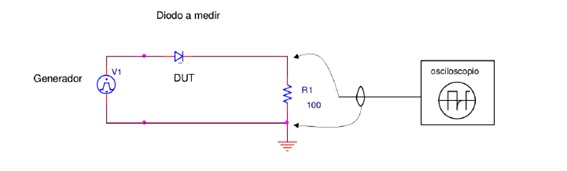
\includegraphics[width=\textwidth]{imagenes/fig1.jpg} 
	\caption{Circuito propuesto para la medición}\label{fig:fig1}
 \end{center}
\end{figure}

Los instrumentos utilizados para efectuar las mediciones fue:
\begin{itemize}\itemsep0em \itemindent=2em
\item Osciloscopio digital de 40 [MHz].
\item Generador de funciones "GW InstexSFG2120".
\item Puntas de osciloscopio compensadas atenuación X10.
\end{itemize}

Los pulsos rectangulares de excitación contaban con una frecuencia de 100 [Hz], y diferentes magnitudes:

\begin{enumerate}[label=(\Alph*)] \itemsep0em \itemindent=2em
\item +5  / 0 [V]
\item +5  /-2 [V]
\item +10 / 0 [V]
\item +10 /-2 [V]
\end{enumerate}

\clearpage

\section{Experiencia}
Sobre cada diodo se aplican las señales propuestas previamente
\subsection{1N5408}
\subsubsection{Señal A}
\begin{figure}[h!]
 \begin{center}
	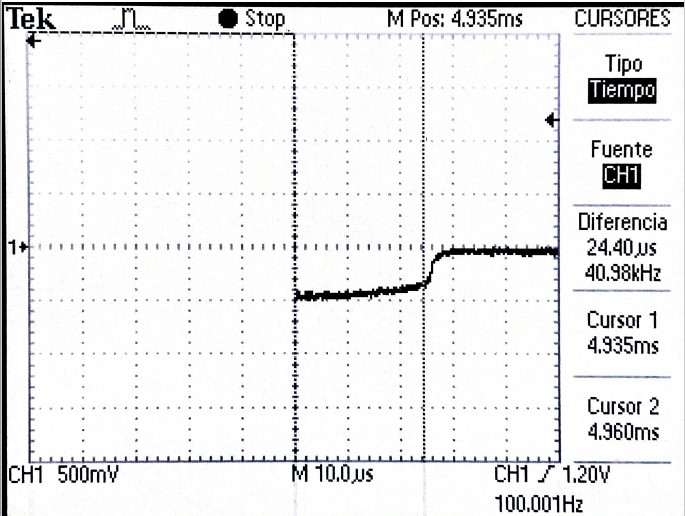
\includegraphics[scale=0.4]{imagenes/1N5408_A.jpg} 
	\caption{Señal A sobre 1N5408}
 \end{center}
\end{figure}
\begin{align*}
	t_{rr} &= 24,4 \; [us] \\
	I_{RM}	&= \frac{V_{RM}}{R} = \frac{500 \; mV}{100 \Omega} = 5 \; [mA] \\
	I_L	&\approx {I_RM} \; \cdot \; t_{rr} = 122 \; [nC]
\end{align*}
%
\subsubsection{Señal B}
\begin{figure}[h!]
 \begin{center}
	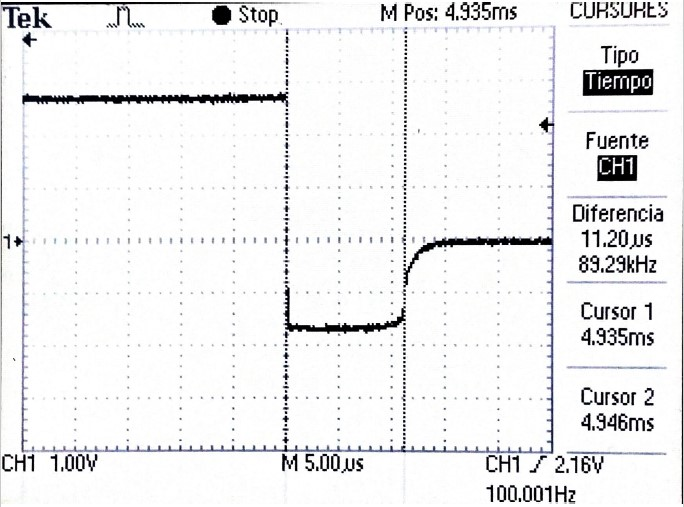
\includegraphics[scale=0.5]{imagenes/1N5408_B.jpg} 
	\caption{Señal B sobre 1N5408}
 \end{center}
\end{figure}
%
\begin{align*}
	t_{rr} &= 11,2 \; [us] \\
	I_{RM}	&= \frac{V_{RM}}{R} = \frac{1,72 \; V}{100 \Omega} = 17,2 \; [mA]\\
	Q_{rr}	&\approx {I_RM} \; \cdot \; t_{rr} = 192,64 \; [nC]
\end{align*}
%
\subsubsection{Señal C}
\begin{figure}[h]
 \begin{center}
	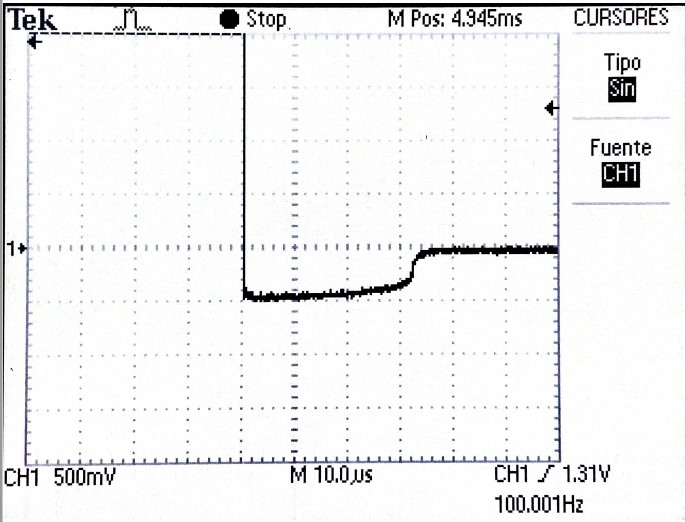
\includegraphics[scale=0.5]{imagenes/1N5408_C.jpg} 
	\caption{Señal C sobre 1N5408}
 \end{center}
\end{figure}
%
\begin{align*}
	t_{rr} &= 30,4 \; [us] \\
	I_{RM}	&= \frac{V_{RM}}{R} = \frac{450 \; mV}{100 \Omega} = 4,5 \; [mA] \\
	Q_{rr}	&\approx {I_RM} \; \cdot \; t_{rr} = 192,64 \; [nC]
\end{align*}
%
\subsubsection{Señal D}
\begin{figure}[h!]
 \begin{center}
	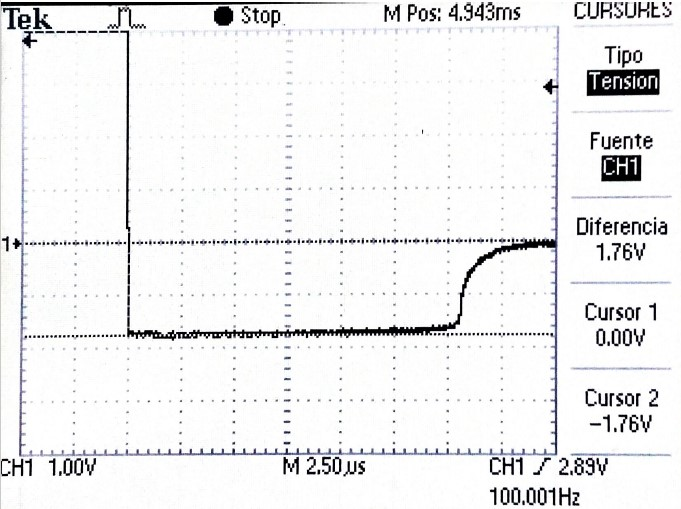
\includegraphics[scale=0.5]{imagenes/1N5408_D.jpg} 
	\caption{Señal D sobre 1N5408}
 \end{center}
\end{figure}
%
\begin{align*}
	t_{rr} &= 15,7 \; [us] \\
	I_{RM}	&= \frac{V_{RM}}{R} = \frac{1,76 \; V}{100 \Omega} = 17,6 \; [mA] \\
	Q_{rr}	&\approx {I_RM} \; \cdot \; t_{rr} = 276,32 \; [nC]
\end{align*}
%
\subsection{MUR160}
\subsubsection{Señal A}
\begin{figure}[h!]
 \begin{center}
	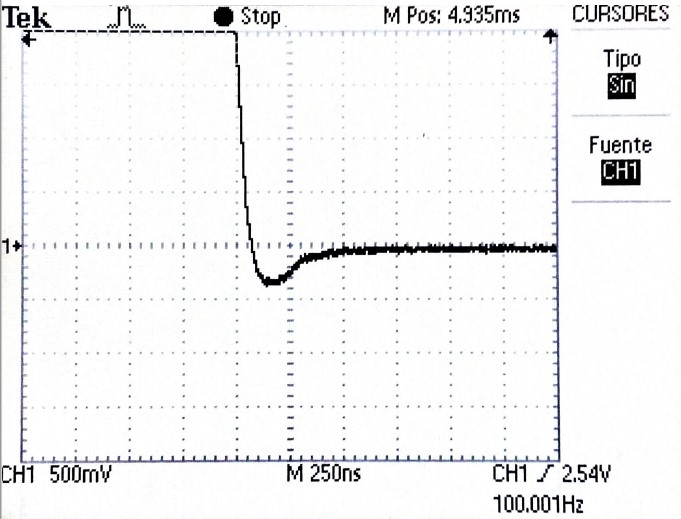
\includegraphics[scale=0.4]{imagenes/MUR_A.jpg} 
	\caption{Señal A sobre MUR160}
 \end{center}
\end{figure}
\begin{align*}
	t_{rr} &= 280 \; [ns] \\
	I_{RM}	&= \frac{V_{RM}}{R} = \frac{340 \; mV}{100 \Omega} = 3,4 \; [mA] \\
	Q_{rr}	&\approx {I_RM} \; \cdot \; t_{rr} = 952 \; [pC]
\end{align*}
%
\subsubsection{Señal B}
\begin{figure}[h!]
 \begin{center}
	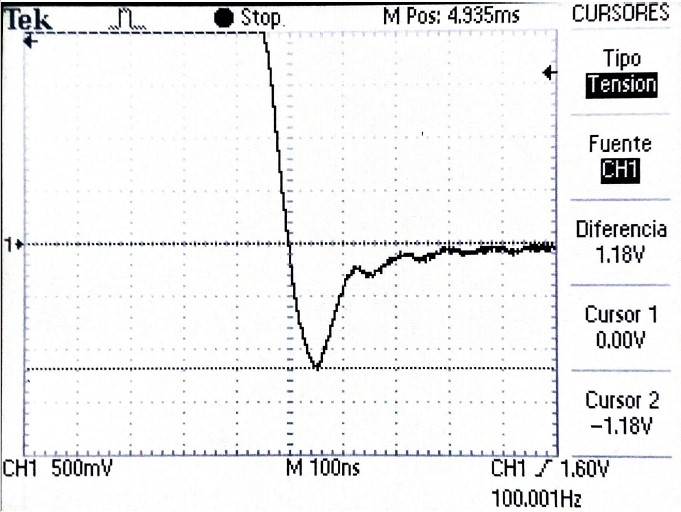
\includegraphics[scale=0.5]{imagenes/MUR_B.jpg} 
	\caption{Señal B sobre MUR160}
 \end{center}
\end{figure}
%
\begin{align*}
	t_{rr} &= 123 \; [ns] \\
	I_{RM}	&= \frac{V_{RM}}{R} = \frac{1,72 \; V}{100 \Omega} = 11,8 \; [mA]\\
	Q_{rr}	&\approx {I_RM} \; \cdot \; t_{rr} = 725,7 \; [pC]
\end{align*}
%
\subsubsection{Señal C}
\begin{figure}[h]
 \begin{center}
	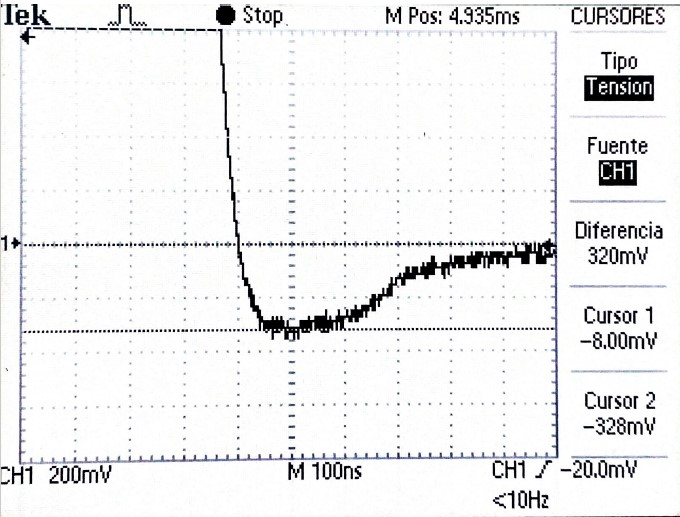
\includegraphics[scale=0.5]{imagenes/MUR_C.jpg} 
	\caption{Señal C sobre MUR160}
 \end{center}
\end{figure}
%
\begin{align*}
	t_{rr} &= 300 \; [ns] \\
	I_{RM}	&= \frac{V_{RM}}{R} = \frac{320 \; mV}{100 \Omega} = 3,2 \; [mA] \\
	Q_{rr}	&\approx {I_RM} \; \cdot \; t_{rr} = 480 \; [pC]
\end{align*}
%
\subsubsection{Señal D}
\begin{figure}[h!]
 \begin{center}
	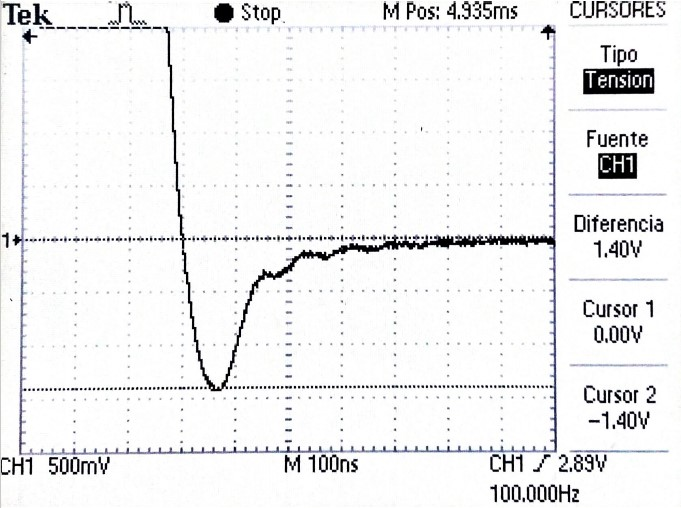
\includegraphics[scale=0.5]{imagenes/MUR_D.jpg} 
	\caption{Señal D sobre MUR160}
 \end{center}
\end{figure}
%
\begin{align*}
	t_{rr} &= 172 \; [ns] \\
	I_{RM}	&= \frac{V_{RM}}{R} = \frac{1,4 \; V}{100 \Omega} = 14 \; [mA] \\
	Q_{rr}	&\approx {I_RM} \; \cdot \; t_{rr} = 1204 \; [nC]
\end{align*}
%
\subsection{1N4148}
Al variar continuamente la escala de tiempo en el osciloscopio se fue profundizando en la forma de onda resultante en la medición. El problema con este diodo, es que no se consiguió estabilizar una forma exacta, la cual dependiendo del movimiento del ajuste del eje temporal experimentaba contracciones y desplazamientos. Todo esto puede entenderse si se toman en cuenta las características dinámicas del dispositivo testeado. Observando la hoja de datos, es notable que el dispositivo por su construcción se considera un diodo rápido (de alta velocidad de recuperación) cuyo $t_{rr}$ (según especificaciones del fabricante) está en el orden de los 4 [ns]. Por tanto, esta situación impulsa a considerar algunas limitaciones; una de ellas es que debido al ancho de banda del osciloscopio está acotado en 50 [Mhz], el mismo no es capaz de captar con la precisión y/o velocidad suficiente, ciertos transitorios o señales variables en ese orden de frecuencia, y por ende se tomarían lecturas erróneas. Por otra parte, el propio generador de funciones empleado, posee un tiempo de bajada (o de cambio general de sus señales) en el orden de los “[ns]”, superando o asemejándose al tiempo de recuperación inversa del diodo, lo que puede y efectivamente ocasiona que el diodo se recupere parcial o totalmente antes que la señal aplicada llegue a su máximo negativo.
Debidas a estas limitaciones, se procedió a realizar un análisis por medio la simulación del dispositivo con el mismo esquema de circuito y excitaciones. El software empleado fue el OrCad versión 17.2 de Cadence.

La figura \textcolor{blue}{\ref{fig:fig2}} muestra el circuito

\begin{figure}[h]
 \begin{center}
	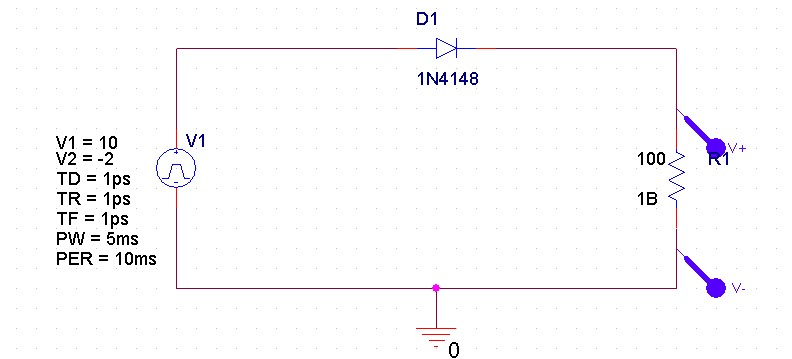
\includegraphics[scale=0.6]{imagenes/fig2.jpg} 
	\caption{Diodo 1N4148 en OrCad Pspice}\label{fig:fig2}
 \end{center}
\end{figure}
%
\subsubsection{Señal A}
\begin{figure}[h!]
 \begin{center}
	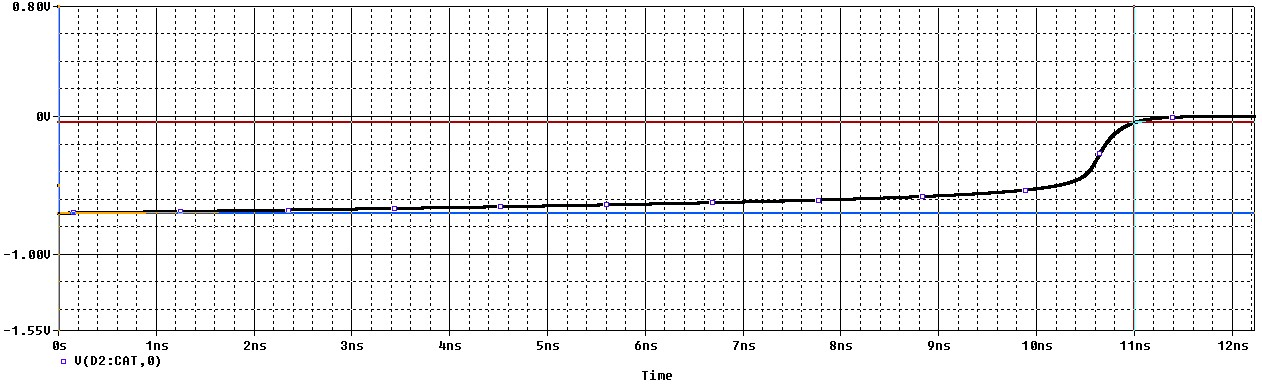
\includegraphics[width=\textwidth]{imagenes/1N4148_A.jpg} 
	\caption{Señal A sobre 1N4148}
 \end{center}
\end{figure}
\begin{align*}
	t_{rr} &= 10,68 \; [ns] \\
	I_{RM}	&= \frac{V_{RM}}{R} = \frac{700 \; mV}{100 \Omega} = 7 \; [mA] \\
	Q_{rr}	&\approx {I_RM} \; \cdot \; t_{rr} = 74,76 \; [pC]
\end{align*}
%
\subsubsection{Señal B}
\begin{figure}[h!]
 \begin{center}
	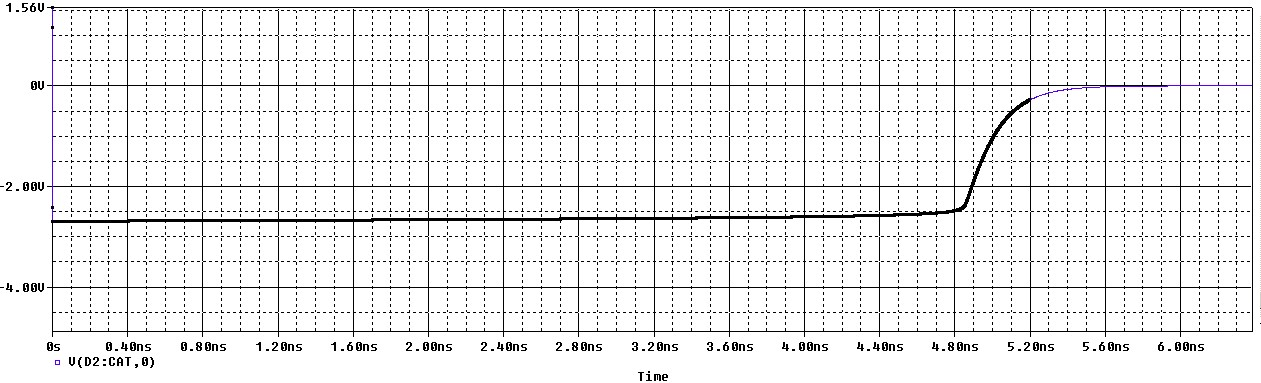
\includegraphics[width=\textwidth]{imagenes/1N4148_B.jpg} 
	\caption{Señal B sobre 1N4148}
 \end{center}
\end{figure}
\begin{align*}
	t_{rr} &= 5 \; [ns] \\
	I_{RM}	&= \frac{V_{RM}}{R} = \frac{2,7 \; V}{100 \Omega} = 27 \; [mA] \\
	Q_{rr}	&\approx {I_RM} \; \cdot \; t_{rr} = 135 \; [pC]
\end{align*}
%
\subsubsection{Señal C}
\begin{figure}[h!]
 \begin{center}
	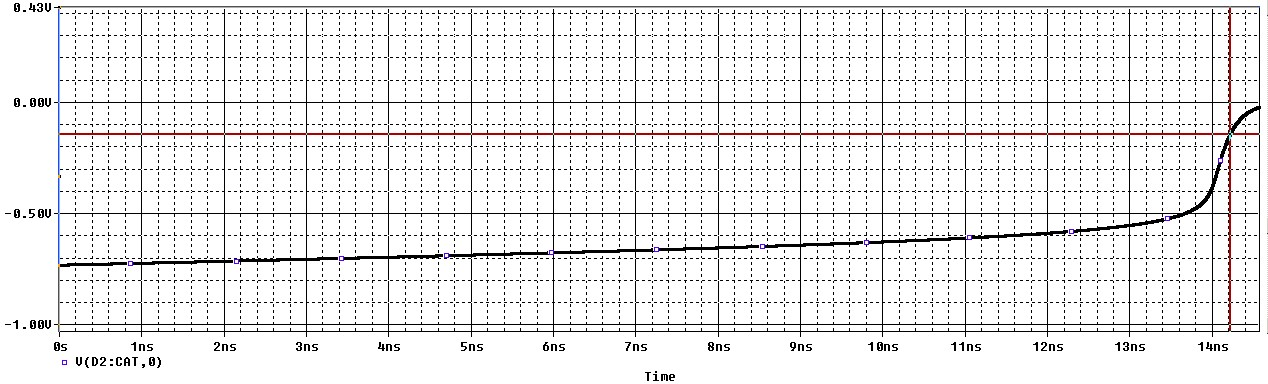
\includegraphics[width=\textwidth]{imagenes/1N4148_C.jpg} 
	\caption{Señal C sobre 1N4148}
 \end{center}
\end{figure}
\begin{align*}
	t_{rr} &= 14,22 \; [ns] \\
	I_{RM}	&= \frac{V_{RM}}{R} = \frac{730 \; mV}{100 \Omega} = 7,3 \; [mA] \\
	Q_{rr}	&\approx {I_RM} \; \cdot \; t_{rr} = 103,806 \; [pC]
\end{align*}
%

\clearpage
\subsubsection{Señal D}
\begin{figure}[h!]
 \begin{center}
	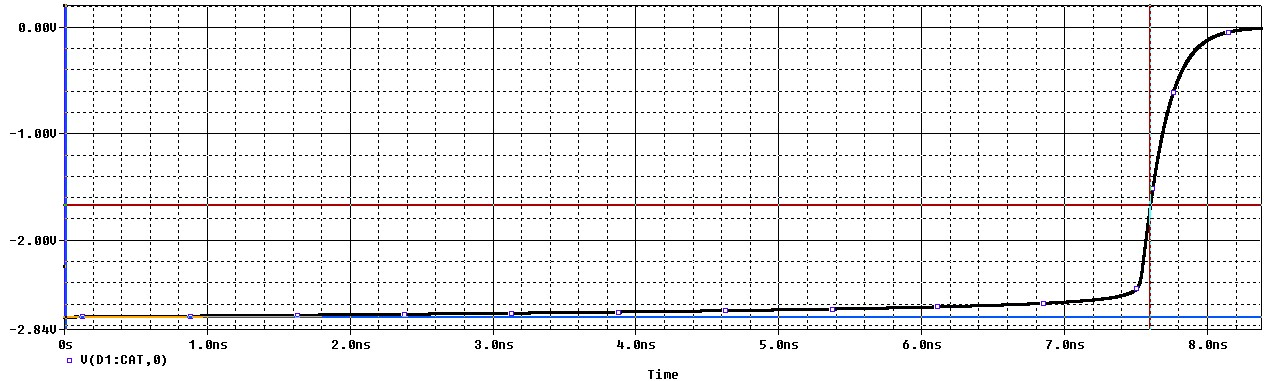
\includegraphics[width=\textwidth]{imagenes/1N4148_D.jpg} 
	\caption{Señal D sobre 1N4148}
 \end{center}
\end{figure}
\begin{align*}
	t_{rr} &= t_a \;+\; t_b = 7,6 \; [ns] + 778 \; [ps] = 8,378 \; [ns] \\
	I_{RM}	&= \frac{V_{RM}}{R} = \frac{2,72 \; V}{100 \Omega} = 27,2 \; [mA] \\
	Q_{rr}	&\approx {I_RM} \; \cdot 7,6 [ns] + \frac{I_{RM}}{2} \cdot 778 \; [ps] = 217,3 \; [pC]
\end{align*}

\section{Tabla comparativa de valores medidos}
A forma de resumen y de una manera más práctica de obtener conclusiones, se presenta la siguiente tabla con los valores medidos en las experiencias anteriormente descritas. 
\begin{center}
\begin{tabular}{ | c | c | c | c | c | c | c |}
  \hline
  	Diodo	&	 \multicolumn{2}{|c|}{1N5408}	&	\multicolumn{2}{|c|}{MUR160}	& \multicolumn{2}{|c|}{1N5408}	\\
  \hline
  Señal		& $t_{rr}$ & $Q_{rr}$ & $t_{rr}$ & $Q_{rr}$ 	& $t_{rr}$ & $Q_{rr}$ \\
  \hline
    A ($5 \; V_{PP}$)	& $24,4 \; [us]$ & $122,00 \; [nC]$	& $280 \; [ns]$ & $952,0 \; [pC]$ & $10,68 \; [ns]$ & $74,760  \; [pC]$ \\
  \hline
    B ($7 \; V_{PP}$)	& $11,2 \; [us]$ & $192,64 \; [nC]$	& $123 \; [ns]$ & $752,7 \; [pC]$ & $5,000 \; [ns]$ & $135,000  \; [pC]$ \\
  \hline
    C ($10 \; V_{PP}$)	& $30,4 \; [us]$ & $136,80 \; [nC]$ & $300 \; [ns]$ & $480,0 \; [pC]$& $14,220 \; [ns]$ & $103,806  \; [pC]$ \\
  \hline
    D ($12 \; V_{PP}$)	& $15,7 \; [us]$ & $276,32 \; [nC]$ & $172 \; [ns]$ & $1204  \; [pC]$ & $8,378 \; [ns]$ & $217,300  \; [pC]$ \\
  \hline
    Datasheet		& $1500 \; [ns]$ & * & 75 [ns] & * & 4 \; [ns] & * \\
  \hline
  
\end{tabular}
\end{center}

\clearpage

\section{Conclusiones}
Según las experiencias realizadas se pueden tomar los siguientes puntos en consideración:
\begin{itemize}
\item[•] Es de suma importancia conocer las características dinámicas del diodo a utilizar según la aplicación. El 1N5408 es adecuado para aplicaciones de rectificación en general, mientras que el MUR160 o el 1N4148 es adecuado para aplicaciones de conmutación rápida.

\item [•] $Q_{rr}$ representa geométricamente el área encerrada de la trayectoria de recuperación inversa del diodo. Físicamente son las cargas recombinadas durante dicho tiempo.

\item [•]	Para todos los circuitos y gráficos resultantes de las mediciones, se observa que con incrementos en los valores pico de las señales aplicadas, se obtiene un mayor valor pico de corriente IRM . Esto es deducible por la Ley de Ohm aplicada a la resistencia, que implica una mayor corriente directa y por tanto mayor cantidad de portadores de carga implicados en dicha corriente. No obstante, dicho aumento de magnitudes (por ejemplo pasar de 5[V] a 10[V]) trae aparejado un pequeño aumento del tiempo de recuperación; pero si además se considera cuando se “forza” más la situación inversa con una tensión negativa, se consigue un notable efecto de reducción en el tiempo $t_{rr}$ de cada diodo respecto a la instancia “sólo positiva anterior”. 

\item [•]Existe una disipación de potencia durante el tiempo de recuperación inversa. Para altas frecuencias, por tanto, se debe usar diodos de recuperación rápida.

\item[•]Se deben tomar en cuenta las limitaciones del instrumental con el que se mide según las prestaciones de los dispositivos. En las experiencias el diodo 1N4148 no pudo ser medido ya que se requería un ancho de banda cinco veces mayor al que el osciloscopio otorga.  En el caso del generador de onda, su tiempo de caída se asemeja al tiempo de recuperación inverso del diodo, lo que indica que el dispositivo se recuperaba anteriormente a lo que el instrumento de medición podría lograr alcanzar su máxima amplitud negativa.

\end{itemize}

\end{document}